
\section{动物学研究的历史}

下面列出部分与动物学有关的历史:

\begin{description}
	\item[动物学之父] 亚里士多德(古希腊);
	\item[现代解剖学之父] 维萨留斯(意大利);
	\item[比较解剖学的先驱] 贝伦(法国博物学家);
	\item[实验医学的鼻祖] 哈维(英国);
	\item[古人的智慧]《夏小正》《尔雅》《梦溪笔谈》《本草纲目》;
	\item[我国现代动物学家] 秉志、蒲蛰龙、江静波、陈世骧、庞雄飞等;
	\item[其他] 马尔比基(意大利)用自制显微镜观察到了血细胞在血管中的流动,支持了哈维的血液循环学说。
\end{description}

\section{动物的基本组织}

动物的组织包括上皮组织、结缔组织、肌肉组织、神经组织。
\begin{figure}[h!]
	\centering
	\begin{forest}
		[动物组织
			[上皮组织]
			[结缔组织]
			[肌肉组织]
			[神经组织]]
	\end{forest}
	\caption{动物组织的分类}
	\label{fig:动物组织的分类}
\end{figure}

\subsection{上皮组织}

上皮组织=密集的细胞+少量的细胞间质,细胞之间还有连接复合体,如桥粒。因为位于表面,所以上皮组织有游离面和基底面之分,即上皮细胞具有极性。

上皮组织包括被覆上皮、腺上皮、感觉上皮。

\subsubsection{被覆上皮}

被覆上皮是覆盖在机体内外表面的上皮组织。按层数分为单层、复层上皮,又可以各自再分为扁平、立方、柱状上皮等。

为了适应不同的功能,有的上皮细胞表面形成纤毛(呼吸道)或微绒毛(近曲小管刷状缘、小肠柱状上皮纹状缘\footnote{即小肠绒毛的微观结构。})

\zhongdian{并非所有无脊椎动物的体表上皮都是单层,也并非所有高等动物体表上皮是复层。}
\begin{table}[h!]
	\centering
	\begin{tabularx}{\textwidth}{|c|X|}
		\hline
		上皮 & \multicolumn{1}{c|}{实例} \\ \hline
		单层扁平上皮 & 内皮:\hspace{-0.5em}心\hspace{-0.25em}、\hspace{-0.5em}血管\hspace{-0.25em}、\hspace{-0.5em}淋巴管;\hspace{-0.5em}间皮:\hspace{-0.5em}腹膜\hspace{-0.25em}、\hspace{-0.5em}胸膜\hspace{-0.25em}、\hspace{-0.5em}心包膜;\hspace{-0.5em}其他:\hspace{-0.5em}肺泡\hspace{-0.25em}、\hspace{-0.5em}肾小囊 \\ \hline
		单层立方上皮 & 甲状腺滤泡、肾小管 \\ \hline
		单层柱状上皮 & 胃、肠、子宫,比较厚,便于形变 \\ \hline
		复层扁平上皮 & 口腔、胃、肠、子宫、阴道、皮肤(角质化了的) \\ \hline
		复层柱状上皮 & 分布范围较窄,仅见于眼睑结膜和男性尿道 \\ \hline
		假复层纤毛上皮 & 呼吸道内表面,在游离面附近有能摆动的纤毛 \\ \hline
		变移上皮 & 膀胱、输尿管道,层数可变,厚度随之变化 \\ \hline
	\end{tabularx}
	\caption{被覆上皮的类型}
	\label{tab:CoveringEpithelium}
\end{table}

\subsubsection{腺上皮}

由具有分泌功能的腺细胞组成,大多为单层立方上皮。

\subsubsection{感觉上皮}

如嗅觉上皮、听觉上皮、视觉上皮、味觉上皮。

\subsection{结缔组织}

结缔组织=细胞+细胞间质。结缔组织包括疏松结缔组织、致密结缔组织、软骨、骨、血液。
\begin{figure}[h!]
	\centering
	\begin{forest}
		[结缔组织
			[疏松结缔组织]
			[致密结缔组织]
			[软骨]
			[骨]
			[血液]]
	\end{forest}
\end{figure}

\subsubsection{疏松结缔组织}

又称蜂窝组织,构成=排列疏松的纤维+分散其中的多种细胞。

含有弹性纤维、胶原纤维、成纤维细胞、巨噬细胞等。纤维较少,基质和细胞较多。

成纤维细胞与纤维细胞是处于不同状态的同种细胞,二者可相互转化。

\subsubsection{致密结缔组织}

致密结缔组织=大量胶原纤维和弹性纤维+少量细胞和基质。

纤维有平行排列和网状交织之分,肌腱、韧带、大动脉管壁的弹性膜的纤维平行排列,真皮层的胶原纤维交织成网。
\subsubsection{脂肪组织}

由大量脂肪细胞聚集而成,疏松结缔组织把细胞分隔成许多脂肪小叶。

脂肪组织分为黄(白)色脂肪组织、米色脂肪组织和褐色脂肪组织。后两者均可主动产热。褐色脂肪组织看起来是褐色就是因为有大量线粒体。三种脂肪组织细胞的结构示意见\autoref{fig:AT}。

\begin{figure}[h!]
	\centering
	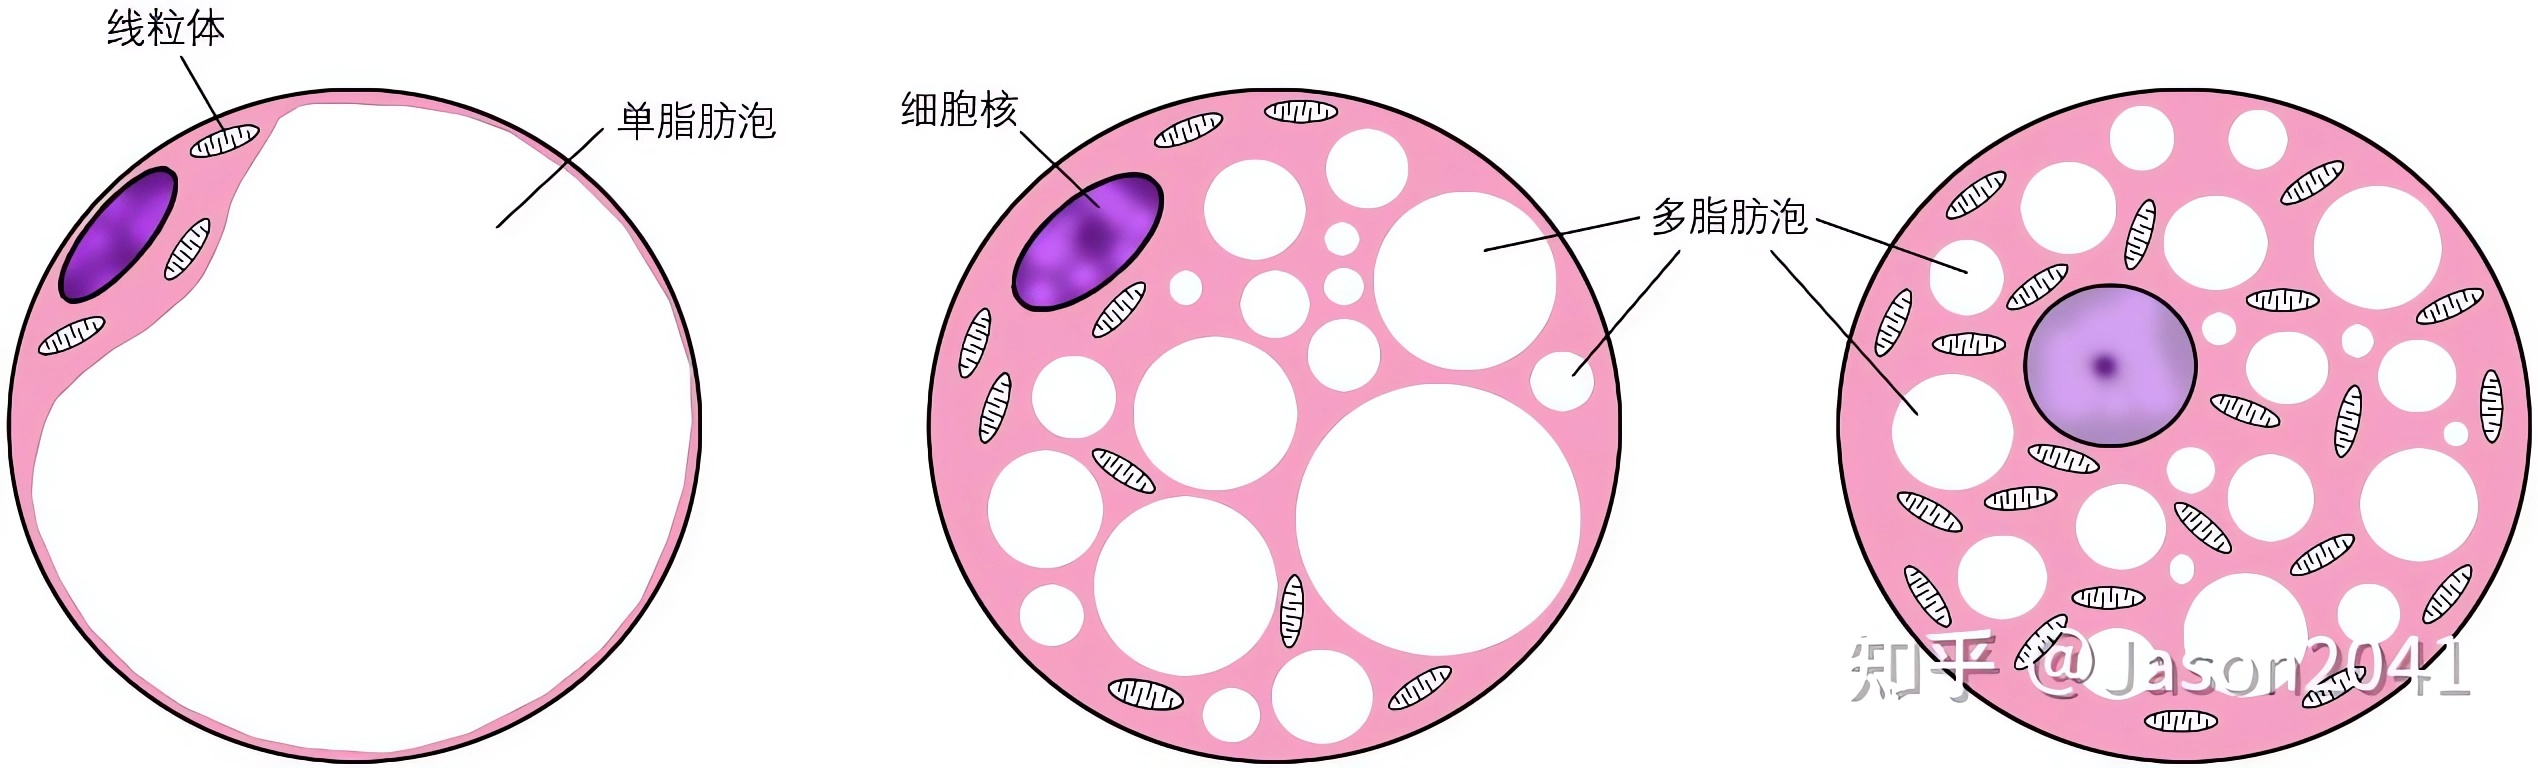
\includegraphics[width=\linewidth]{脂肪组织}
	\caption{白色、米色、褐色脂肪组织的示意图}
	\label{fig:AT}
\end{figure}


\subsubsection{网状组织}

分布于造血器官,构成淋巴细胞和血细胞发育的微环境。

\subsubsection{软骨组织}

软骨组织=软骨细胞+纤维+基质。根据纤维的性质分为透明软骨、纤维软骨、弹性软骨。软骨里没有血管分布。透明软骨基质中有陷窝。人的弹性软骨终生不钙化。

\begin{table}[h!]
	\centering
	\begin{tabularx}{\textwidth}{|c|C|c|}
		\hline
		软骨 & 分布 & 纤维 \\ \hline
		透明软骨 & 最广,关节、肋、气管 & 胶原纤维 \\ \hline
		纤维软骨 & 椎间盘、关节盂 & 胶原纤维 \\ \hline
		弹性软骨 & 耳廓、会厌 & 弹力纤维 \\ \hline
	\end{tabularx}
	\caption{三种软骨的特征}
	\label{tab:3Cartilage}
\end{table}


\subsubsection{骨组织}

骨组织=骨细胞+骨胶纤维+基质。

骨髓是造血器官,形成各种血细胞。体内钙的储存库。

骨分密质骨和松质骨,区别如\autoref{tab:bones}所示。

\begin{table}[htbp]
	\centering
	\begin{NiceTabularX}{\textwidth}{cXX}[hvlines]
		特征 & \Block[c]{1-1}{\textbf{密质骨}} & \Block[c]{1-1}{\textbf{松质骨}} \\
		\Block[v-center]{1-1}{结构} & 骨板紧密排列,骨胶纤维平行排列 & 网状,空隙较大,有骨髓 \\
		\Block[v-center]{1-1}{骨细胞} & 具有多个突起,通过细管连接 & 不如密质骨密集 \\
		\Block[v-center]{1-1}{血管} & 哈氏管内含血管和神经,形成网络 & 主要通过骨髓获取血液供应 \\
		\Block[v-center]{1-1}{位置} & 表面/环骨髓腔 & 长骨的骺端、短骨和不规则骨内部 \\
		\Block[v-center]{1-1}{功能} & 强度和结构支持 & 轻质支持,储存骨髓参与造血 \\
	\end{NiceTabularX}
	\caption{密质骨和松质骨的对比}
	\label{tab:bones}
\end{table}

\subsubsection{血液}

略,有关内容见生理学。

\subsection{肌肉组织}

略,有关内容见生理学。

\subsection{神经组织}

神经细胞胞质内有尼氏小体,嗜碱性染料,实际上是成堆的糙面内质网。它只存在于树突,而不存在于轴突、轴丘\footnote{轴丘是轴突起源的地方。}。

\section{原生动物门}

\subsection{原生动物的一般特征}

\subsubsection{形态结构}

绝大多数都是微小的单细胞生物,但也有较大者如部分有孔虫。有些原生动物形成多细胞群体,如盘藻、杂球藻等。

原生动物身体表面的情况如下述:
\begin{itemize}
	\item 无固定形态,很薄的原生质膜,如变形虫;
	\item 有固定的体型,
	\begin{itemize}
		\item 眼虫的细胞膜形成皮膜,具有厚度和弹性,可以轻微变形;
		\item 衣滴虫形成了类似植物细胞壁的结构,无法变形。
	\end{itemize}
\end{itemize}

原生动物的身体形状随生活方式而变化:(\autoref{tab:protozoanBodyShapeAndLifestyleRelationship})

\begin{table}[htbp]
	\centering
	\begin{tabularx}{\textwidth}{|c|X|l|}
		\hline
		\textbf{生活方式} & \multicolumn{1}{c|}{\textbf{特点}} & \multicolumn{1}{c|}{\textbf{举例}} \\ \hline
		固着生活 & 锥形、球形,具肌动蛋白的柄可收缩 & 钟形虫、足吸管虫 \\ \hline
		漂浮生活 & 球形,具伪足 & 辐球虫、某些有孔虫 \\ \hline
		游泳生活 & 梭形 & 草履虫 \\ \hline
		底栖爬行 & 扁形,腹面纤毛形成棘毛 & 棘尾虫 \\ \hline
		寄生生活 & 失去了鞭毛或鞭毛形成波动膜 & 前者利什曼原虫,后者锥虫 \\ \hline
	\end{tabularx}
	\caption{原生动物体形与生活方式的关系}
	\label{tab:protozoanBodyShapeAndLifestyleRelationship}
\end{table}

一些原生动物可以分泌形成外壳,如薄甲藻、表壳虫、砂壳虫、有孔虫、放射虫。

原生动物的细胞质分为外质和内质。外质透明、较致密,内质不透明、含有颗粒。在变形虫中可清晰观察到外质和内质的转化。

\mbox{}

传统上把原生动物如下分类:(\autoref{fig:classificationProtozoan})

\begin{figure}[htbp]
	\centering
	\begin{forest}
		forest scheme
		[原生动物
			[鞭毛虫纲
				[植鞭亚纲]
				[动鞭亚纲]]
			[肉足虫纲]
			[孢子虫纲]
			[纤毛虫纲]]
	\end{forest}
	\caption{原生动物的分类}
	\label{fig:classificationProtozoan}
\end{figure}

\subsection{鞭毛虫纲}

鞭毛虫纲均具鞭毛。分为植鞭亚纲和动鞭亚纲(\autoref{tab:phytomastiginaAndZoomastiginaComparison})。

\begin{table}[htbp]
	\centering
	\begin{tabularx}{\textwidth}{|c|C|C|}
		\hline
		亚纲 & \textbf{植鞭亚纲} & \textbf{动鞭亚纲} \\ \hline
		体表 & 细胞壁或皮膜 & 细胞膜 \\ \hline
		营养 & 具色素体,可自养 & 异养 \\ \hline
		食物贮存 & 淀粉粒、副淀粉粒 & 糖原 \\ \hline
		生殖 & 有性、无性 & 仅无性 \\ \hline
		鞭毛 & 通常为2 & 不定 \\ \hline
		生活 & 自由生活 & 多数寄生或共生 \\ \hline
	\end{tabularx}
	\caption{植鞭亚纲和动鞭亚纲的比较}
	\label{tab:phytomastiginaAndZoomastiginaComparison}
\end{table}

\subsection{纤毛虫纲}

\subsubsection{纤毛虫纲的一般特征}

\paragraph{形态结构}

绝大多数纤毛虫自由生活,少数寄生、共生或固着生活。

\section{胚胎发育}

多细胞动物具有胚胎发育过程,早期胚胎发育的几个过程是相同的。
胚胎发育的重要阶段:受精卵$\longrightarrow$卵裂$\longrightarrow$桑椹胚$\longrightarrow$囊胚$\longrightarrow$原肠胚$\longrightarrow$分化出中胚层$\longrightarrow$神经胚
\subsection{卵细胞}

卵细胞内有大量\sy{卵黄},根据卵黄多少将卵分为少黄卵、中黄卵、多黄卵。


\subsection{卵裂}

卵裂的特点是分裂球总体积保持不变,新分裂的细胞不长大,分裂出的细胞越来越小。

卵裂的方式与卵黄多少有关



文昌鱼前2\textasciitilde3对体节中,体腔来源于肠体腔;后面体节中来源于裂体腔。


\subsection{各胚层分化}

胚层分化列于\autoref{tab:germLayerDifferentiation}中.

\begin{table}[htbp]
	\centering
	\begin{NiceTabularX}{\textwidth}{cccX}[hvlines]
		胚层 &  &  & \Block[c]{1-1}{器官或组织} \\
		\Block{3-1}{外胚层} & \Block[v-center]{1-1}{体壁外胚层} & \Block[v-center]{1-1}{---} & 表皮、消化管两端、表皮衍生物、感觉上皮、眼的晶体、垂体前叶(腺垂体)、牙釉质、除圆口类外脊椎动物的鳃 \\
		& \Block{2-1}{神经外胚层} & \Block[v-center]{1-1}{神经管} & 脑和脊髓、传出神经、视网膜、视神经、垂体后叶(神经垂体) \\
		&  & \Block[v-center]{1-1}{神经嵴} & 脊神经节、传入神经、植物性神经、肾上腺髓质、鳃部骨骼及衍生物、色素细胞、头部真皮 \\
		\Block{9-1}{中胚层} & 脊索中胚层 & --- & 脊索 \\
		& \Block{3-1}{上节} & 生皮节 & 真皮 \\
		&  & 生肌节 & 骨骼肌 \\
		&  & 生骨节 & 脊柱 \\
		& \Block{2-1}{中节} & 生肾节 & 排泄系统 \\
		& & 生殖嵴 & 大部分生殖系统\\
		& \Block{2-1}{下节} & 体壁中胚层 & 腹膜、部分骨骼肌 \\
		&  & \Block[v-center]{1-1}{脏壁中胚层} & 脏膜(浆膜)、肠系膜、循环系统、血液、生殖细胞、平滑肌、部分骨骼肌 \\
		& \Block[v-center]{1-1}{间充质} & \Block[v-center]{1-1}{---} & 主要来源于中胚层,有时也有神经嵴和内胚层。有很强的全能性,可以分化为全部结缔组织 \\
		\Block[v-center]{1-1}{内胚层} & \Block[v-center]{1-1}{---} & \Block[v-center]{1-1}{---} & 原肠及其衍生物(注意两端来源于外胚层),即消化道内层上皮(黏膜层)、消化腺、气管和肺的内层、膀胱和尿道内层、大部分内分泌腺(甲状腺、甲状旁腺、胸腺)、扁桃体 、咽囊、圆口类的鳃 \\
	\end{NiceTabularX}
	\caption{各胚层分化}
	\label{tab:germLayerDifferentiation}
\end{table}

\section[多孔动物门]{多孔动物门(海绵动物门)}

多孔动物可以说是最原始的多细胞动物\footnote{当然有人认为中生动物才是最原始的多细胞动物。}。从前认为这类动物在演化上是一个侧支,但现在发现并不是。

海绵遍布全世界,主要生活在海水中,只有一科生活在淡水中。

\subsection{多孔动物总述}

\subsubsection{体制}

海绵的体型大多数不规则,少数是辐射对称。海绵体表有无数小孔,水流从这里出入,带入氧气、事物。排出废物。

\subsubsection{细胞与组织}

海绵的体壁由两层细胞构成,两层细胞之间为中胶层。

\begin{table}[htbp]
	\centering
	\begin{tabularx}{\textwidth}{|c|C|C|}
		\hline
		体壁 & 细胞或结构 & 功能 \\ \hline
		\multirow{3}{*}{外层} & 扁细胞 & 保护、(有肌丝)收缩 \\ \cline{2-3}
		& 肌细胞 & 控制水流 \\ \cline{2-3}
		& 孔细胞 & 形成入水小孔 \\ \hline
		\multirow{6}{*}{中胶层} & 钙质或硅质的骨针 & 支持 \\ \cline{2-3}
		& 类蛋白质的海绵丝 & 支持 \\ \cline{2-3}
		& 成骨针细胞 & 分泌骨针 \\ \cline{2-3}
		& 成海绵质细胞 & 分泌海绵质纤维 \\ \cline{2-3}
		& 原细胞 & 具全能性 \\ \cline{2-3}
		& 芒状细胞 & 神经传导 \\ \hline
		内层 & 领细胞(单沟系海绵) & 有鞭毛和领,滤食 \\ \hline
	\end{tabularx}
	\caption{海绵动物各层细胞}
	\label{tab:sponge_cells}
\end{table}

中胶层内的成骨针细胞、成海绵质细胞、原细胞统称变形细胞。领细胞行细胞内消化,在领细胞内或是传给变形细胞消化。消化后的残渣还是交回给领细胞排到水流中带走\footnote{刘凌云老师的《普通动物学(第4版)》此处有误。}。

淡水生活的海绵,细胞内还有伸缩泡。

海绵动物细胞分化较多,细胞间有些联系,却又不是紧密协作。它们还没形成明确的组织。

\subsubsection{水沟系}

\begin{figure}[h]
	\centering
	\begin{forest}
		[水沟系
			[单沟型]
			[双沟型]
			[复沟型]]
	\end{forest}
\end{figure}

\begin{table}[htbp]
	\centering
	\begin{tabularx}{\textwidth}{|c|c|C|c|}
		\hline
		类型 & 领细胞分布 & 水流路径 & 举例 \\ \hline
		单沟型 & 中央腔壁 & 入水小孔$\longrightarrow$中央腔$\longrightarrow$出水口 & 白枝海绵 \\ \hline
		双沟型 & 辐射管壁 & 流入孔$\longrightarrow$流入管$\longrightarrow$前幽门孔$\longrightarrow$辐射管$\longrightarrow$后幽门孔$\longrightarrow$中央腔$\longrightarrow$出水口 & 毛壶 \\ \hline
		复沟型 & 鞭毛室 & 流入孔$\longrightarrow$流入孔$\longrightarrow$前幽门孔$\longrightarrow$鞭毛室$\longrightarrow$后幽门孔$\longrightarrow$流出管$\longrightarrow$中央腔$\longrightarrow$出水口 & 浴海绵、淡水海绵 \\ \hline
	\end{tabularx}
	\caption{海绵水沟系的类型}
	\label{tab:sponge_canal}
\end{table}

双沟型海绵相当于单沟型海绵的体壁折叠形成。复沟型海绵的中央腔壁由扁细胞构成。
\section{腔肠动物门}

\section{扁形动物门}

\begin{gs}[:毛泽东《送瘟神》]
	1958年7月1日,毛主席在得知江西余江县消灭了血吸虫病之后,作诗二首:

	\mbox{}

	\fangsong
	\hspace{2em} 读六月三十日《人民日报》,余江县消灭了血吸虫。浮想联翩,夜不能寐。微风拂煦,旭日临窗,遥望南天,欣然命笔。
	\begin{center}
		\kaishu
		绿水青山枉自多,华佗无奈小虫何!\\
		千村薜荔人遗矢,万户萧疏鬼唱歌。\\
		坐地日行八万里,巡天遥看一千河。\\
		牛郎欲问瘟神事,一样悲欢逐逝波。\\

		\mbox{}

		春风杨柳万千条,六亿神州尽舜尧。\\
		红雨随心翻作浪,青山着意化为桥。\\
		天连五岭银锄落,地动三河铁臂摇。\\
		借问瘟君欲何往,纸船明烛照天烧。\\

	\end{center}
\end{gs}

\section{假体腔动物门}

\section{节肢动物门}

\begin{table}[htbp]
	\centering
	\begin{tabularx}{\textwidth}{|c|c|c|X|}
		\hline
		体区 & 序号 & 名称 & \multicolumn{1}{c|}{功能} \\ \hline
		\multirow{5}{*}{头部} & 1 & 小触角 & 嗅觉、平衡、触觉(前部) \\ \cline{2-4}
		& 2 & 大触角 & 触觉(两侧、后部) \\ \cline{2-4}
		& 3 & 大颚 & 咀嚼食物 \\ \cline{2-4}
		& 4 & 第一小颚 & 抱握食物 \\ \cline{2-4}
		& 5 & 第二小颚 & 外肢形成呼吸板 \\ \hline
		\multirow{4}{*}{胸部} & 6 & 第一颚足 & 具鳃 \\ \cline{2-4}
		& 7 & 第二颚足 & 具鳃 \\ \cline{2-4}
		& 8 & 第三颚足 & 具鳃 \\ \cline{2-4}
		& 9-13 & 步足 & 捕食、爬行(前3对末端钳状,后2对爪状) \\ \hline
		\multirow{2}{*}{腹部} & 14-18 & 游泳足 & 游泳。雄虾第1腹肢内肢特化成交接器 \\ \cline{2-4}
		& 19 & 尾足 & 强大,增强拨击逃避 \\ \hline
	\end{tabularx}
	\caption{中国对虾的附肢}
	\label{tab:AppendagesOfChineseShrimp}
\end{table}

\begin{table}[htbp]
	\centering
	\begin{tabularx}{\textwidth}{|c|C|C|C|C|}
		\hline
		\textbf{类别} & \textbf{口器} & \textbf{前翅} & \textbf{后翅} & \textbf{变态} \\ \hline
		直翅目 & 咀嚼 & 革 & 膜 & 渐 \\ \hline
		半翅目 & 刺吸 & 半鞘 & 膜 & 渐 \\ \hline
		同翅目 & 刺吸 & 膜质或无 & 膜质或无 & 渐 \\ \hline
		鳞翅目 & 虹吸 & 鳞翅 & 鳞翅 & 完全 \\ \hline
		鞘翅目 & 咀嚼 & 鞘 & 膜 & 完全 \\ \hline
		膜翅目 & 咀嚼或嚼吸 & 膜质或无 & 膜质或无 & 完全 \\ \hline
		双翅目 & 刺吸或舐吸 & 膜 & 平衡棒 & 完全 \\ \hline
		蜻蜓目 & 咀嚼 & 膜 & 膜 & 半 \\ \hline
	\end{tabularx}
	\caption{昆虫重要纲的特征对比}
	\label{tab:insect_speciality}
\end{table}

脊索动物大多数内容都在最后比较解剖部分叙述,此处仅补充介绍分类、起源等。

\section{尾索动物亚门}

\section{头索动物亚门}

\section{圆口纲}

\section{鱼纲}

\subsection{鱼纲的主要特征}

\subsubsection{外形}

\begin{itemize}
	\item 软骨鱼类,头和躯干以最后一对鳃裂为界,躯干和尾以泄殖腔孔为界。口在腹面,横裂;
	\item 硬骨鱼类,头和躯干以鳃盖后缘为界,躯干和尾以肛门和泄殖孔为界。
\end{itemize}

硬骨鱼口的位置分为
\begin{description}
	\item[端位] 多数种类,如鲤、鲫、\xpinyin*{鳢};
	\item[上位] 中上层鱼类,如鲢、鳙;
	\item[下位] 中下层鱼类,如鲟、鳇、泥鳅。
\end{description}
由此可见鱼口“结构与功能相适应”的特点。

硬骨鱼躯干两侧各有一条侧线,这是由埋在皮肤内的侧线管开口在体表的小孔形成。被侧线穿过的鳞叫侧线鳞,于是,鱼的鳞式是这样表示的:
\[\text{侧线鳞数}\frac{\text{侧线上鳞数}}{\text{侧线下鳞数}}\]


\subsection{鱼纲的分类}
